\section{Electronics}

electronic sensors basically consist of three parts

change in some physical property (temperature, pressure, etc.) is picked up by a \keypoint{sensor}

electrical signal is then fed to \keypoint{processing units}

processor produces an output voltage to drive \keypoint{output devices} to indicate this change

\subsection{sensors}

\subsubsection{thermistor}

\begin{wrapfigure}{r}{0.45\textwidth}
	\centering
		\begin{circuitikz}[european resistors]
		\draw[thick] (0,0) to [thR,l_=$R_T$] (3,0);
	\end{circuitikz}
	\caption*{electric symbol for thermistor}
	
	\vspace*{\baselineskip}
	\begin{tikzpicture}[scale=0.8]
	\draw[->] (-1.6,0) -- (5,0) node[below] {$T$/\OC};
	\draw[->] (0,0) node[below]{0} -- (0,4) node[above] {$R_T$};
	\draw[blue,thick] (-1.5,4) [out=-60,in=170] to (4.8,0.8);
	\end{tikzpicture}
\end{wrapfigure}

\keypoint{thermistor}\index{thermistor} is an electrical component with a resistance that varies with temperature

thermistors usually have a \emph{negative temperature coefficient}, or NTC in short,  which means their resistance decreases as temperature rises

in A-Levels, we consider NTC thermistors only

\cmt resistance-temperature relation is \emph{non-linear}
	
if a graph is sketched, the curve looks like an exponential decay
	
\cmt behaviour of NTC thermistors can be explained in terms of \emph{band theory} (see \S\ref{band-theory})

at low temperature, electrons are bound to atoms and cannot move freely; at high temperature, electrons gain energy and break free from atoms, so more free electrons available to conduct electricity

\subsubsection{LDR}

\begin{wrapfigure}{r}{0.4\textwidth}
	\vspace*{-16pt}
	\centering
	\begin{circuitikz}[european resistors]
		\draw[thick,->] (1.6,0.6) -- ++(-.3,-.3);
		\draw[thick,->] (1.8,0.6) -- ++(-.3,-.3);
		\draw[thick] (0,0) to [R,l_=LDR] (3,0);
	\end{circuitikz}
	
	\caption*{electric symbol for LDR}
	
	\vspace*{\baselineskip}
	\begin{tikzpicture}[scale=0.84]
	\draw[->] (0,0) -- (5,0) node[below left] {$I$};
	\draw[->] (0,0) node[below]{0} -- (0,4) node[above] {LDR};
	\draw[blue,thick] (-0,3.6) [out=-75,in=170] to (4.8,0.8);
	\end{tikzpicture}
\end{wrapfigure}

	

\keypoint{light-dependent resistor}, or \keypoint{LDR}\index{LDR}, is an electrical component with a resistance that can change with intensity of light

resistance of LDR decreases as light level increases

\cmt resistance of LDR varies \emph{non-linearly} with intensity

\cmt behaviour of LDR is also explained with \emph{band theory}

bound electrons acquire energy from radiation and become conducting, greater light intensity means more free electrons available

\cmt in dark, typical resistance of LDR $\approx10^5\sim10^7$ $\Omega$

in bright, typical resistance of LDR $\approx10^2\sim10^3$ $\Omega$


\subsubsection{strain gauge}

\begin{wrapfigure}{r}{0.4\textwidth}
	\centering
	\begin{tikzpicture}[scale=0.75,rotate=30]
	\draw[thick,fill=blue!15,rounded corners] (-2,0) rectangle (3.2,2.4);
	\foreach \x in {0.3,0.7,1.1,1.5} \draw[very thick] (0.3,\x) --++ (2.4,0) arc(-90:90:0.1) --++ (-2.4,0) arc (270:90:0.1);
	\draw[very thick] (0.3,1.9) --++ (2.4,0) arc(-90:90:0.1) --++ (-2.4,0);
	\draw[very thick] (0.3,0.3) [out=180, in=0] to (-2,0.6) --++ (-2,0);
	\draw[very thick] (0.3,2.1) [out=180, in=0] to (-2,1.8) --++ (-2,0);
	\draw (-3,0.5) --++ (-.924,-1.6) node[below,twoline]{connection\\leads};
	\draw (1.8,0.2) --++ (-.924,-1.6) node[below,twoline]{metal\\wire};
	\draw (3,2.1) --++ (-1,1.6) node[above,twoline]{plastic\\sheet};
	\end{tikzpicture}
	
	\caption*{structure of a strain gauge}
\end{wrapfigure}

to measure width of a narrow crack, a device called \keypoint{strain gauge}\index{strain gauge} is widely used in industry

a metal-wire strain gauge consists of a folded long wire sealed on a thin plastic box

as crack widens, strain gauge gets stretched, length of wire increases, causing a change in its resistance

resistance of a metal wire is given by: $R=\frac{\rho l}{A}$

increase in resistance is proportional to increase in length of wire (for small increments)

\cmt if change in cross-sectional area of wire is negligible

increase in resistance: $\Delta R = \frac{\rho\Delta l}{A} \ra \boxed{\frac{\Delta R}{R} = \frac{\Delta l}{l}}$

\cmt if cross-sectional area of wire changes with its length

total volume of wire $V=Al$ should remain constant

it can be shown that
\footnote{To keep $V=Al$ constant, for small change in $l$, one has $\frac{\Delta A}{A} \approx \frac{\Delta l}{l}$. Resistance of the stretched wire is: $R+\Delta R = \frac{\rho(l+\Delta l)}{A-\Delta A} = \frac{\rho l}{A} \left(1 + \frac{\Delta l}{l}\right) \left(1 - \frac{\Delta A}{A}\right)^{-1} \approx R \left(1 + \frac{\Delta l}{l}\right) \left(1 - \frac{\Delta l}{l}\right)^{-1}$. For $x\ll1$, we can use binomial expansion $(1+x)^n = 1 + nx + \cdots$. Drop higher order terms, we find to the first-order approximation that: $R+\Delta R \approx R \left(1 + \frac{\Delta l}{l}\right) \left(1 + \frac{\Delta l}{l}\right) \approx R\left( 1 + \frac{2\Delta l}{l}\right)$, so $\Delta R = 2R\frac{\Delta l}{l}$, it then follows that $\frac{\Delta R}{R} = \frac{2\Delta l}{l}$.}
 the percentage increase in resistance is: $\boxed{\frac{\Delta R}{R} = \frac{2\Delta l}{l}}$

notice the differences, change in length causes increase in resistance, reduction in cross section makes the same contribution, hence an extra factor of two.

\subsubsection{piezo-electric transducer}\label{ch-piezo}

\keypoint{piezo-electric transducer}\index{piezo-electric transducer} transforms mechanical energy into electrical energy, or vice versa

when a piezo-electric material\footnote{Materials that exhibit piezo-electricity include quartz, certain ceramics, various proteins, etc.} is compressed, a p.d. is produced across it

conversely, p.d applied across piezo-electric material can cause change in shape

since its discovery, piezo-electricity was exploited in many useful applications



\cmt piezo-electric transducer can be used to generate sound waves

apply an a.c. voltage, material is forced to vibrated at same frequency as a.c.

this causes compression and rarefaction of air, producing sound waves

so piezo-electric transducer is the key component in \emph{loudspeakers} and \emph{buzzers}

\cmt piezo-electric transducer can also be used to detect sound waves

exposed to sounds, variation in air pressure produces an a.c. voltage across the device

this signal can be measured and processed to represent original sound wave

so piezo-electric transducer is also found in \emph{microphones}

\begin{figure}[ht]
	\centering
	\begin{minipage}{0.45\textwidth}
		\centering
		\begin{circuitikz}
			\draw (0,0) to[mic] ++(0,1.8);
		\end{circuitikz}
		\caption*{symbol for a microphone}
	\end{minipage}
	\begin{minipage}{0.45\textwidth}
		\centering
		\begin{circuitikz}
			\draw (0,0) to[loudspeaker] ++(0,-1.8);
		\end{circuitikz}
		\caption*{symbol for a loudspeaker}
	\end{minipage}
\end{figure}

\cmt mechanism of piezo-electricity is explained on molecular level
	
piezo-electric materials consist of \emph{polarised} molecules, also called \emph{dipoles}
	
when being compressed, dipoles rearrange themselves, causing variation of charge density, so small voltage is generated (see illustration)
	
\begin{figure}[ht]
	\vspace*{-10pt}
	\centering
	\includegraphics[height=160pt]{piezo-electric.pdf}
		%\caption{nature of piezo-electricity due to dipole structure}
	\vspace*{-10pt}
\end{figure}
	




\subsection{processors}

\subsubsection{potential divider}

sensors such as thermistor and LDR only produce changes in resistance, but output devices are driven by voltages $\longrightarrow$ \keypoint{potential divider} circuit can be used

a potential divider consists of two resistors in series connected to a fixed voltage supply

\begin{wrapfigure}{r}{0.32\textwidth}
	\vspace{-15pt}
	\centering
	\begin{center}
		\begin{circuitikz}[european resistors,yscale=.8,xscale=1.1]
			\draw[thick] (0,5) -- (2,5) to [R,l_=$R_1$] (2,2.5) to [R,l_=$R_2$] (2,0) -- (1,0) node[ground]{} -- (0,0);
			\draw[thick,->] (0.5,0) -- (0.5,5) node[left,midway]{$V_0$};
			\foreach \h in {0,2.5,5} \draw[thick] (2,\h) -- ++(1,0);
			\draw[thick,<->] (2.7,2.5) -- ++ (0,2.5) node[midway,right]{$V_1$};
			\draw[thick,<->] (2.7,0) -- ++ (0,2.5) node[midway,right]{$V_2$};
			\node[left] at (2,2.5) {$X$};
		\end{circuitikz}
	\end{center}
	\vspace{-15pt}
\end{wrapfigure}

voltage is shared between the resistors: $V_0 = V_1 + V_2$

p.d. across each resistor: $V_1 = IR_1$, $V_2 = IR_2$

but same current $I$ flows through $R_1$ and $R_2$, so $\boxed{\frac{V_1}{V_2} = \frac{R_1}{R_2}}$

this shows voltage is shared in proportion to resistance

for each resistor: $\boxed{V_1 = \frac{R_1}{R_1+R_2}V_0}, \, \boxed{V_2 = \frac{R_2}{R_1+R_2}V_0}$

\cmt if $R_1$ increases, while $R_2$ is fixed, then $V_1\up$, $V_2 \down$

if $R_1$ decreases, while $R_2$ is fixed, then $V_1\down$, $V_2 \up$

\cmt sometimes we need specify \emph{electric potential} at a given point

potential at any point is measured with respect to a reference point

this point is called \keypoint{earth} or \keypoint{ground}, with a potential defined to be zero

for example, potential at $X$ is essentially equal to voltage $V_2$



\begin{wrapfigure}{r}{0.35\textwidth}
	\vspace{-10pt}
	\centering
	\begin{circuitikz}[european resistors,yscale=1.2]
		\draw[thick,->] (0.58,1.1) -- ++(-.3,-.3);
		\draw[thick,->] (0.58,1.3) -- ++(-.3,-.3);
		\draw[thick] (-2,4)node[left] {$+V_0$} -- (0,4) to [R,l_=$R_0$] (0,2) to [R,l_=LDR] (0,0) -- (-1,0) node[ground]{} -- (-2,0);
		\draw[thick] (0,0) -- (2,0);
		\draw[thick] (0,2) -- (2,2);
		\draw[thick,<->] (1.5,0) -- (1.5,2) node[midway,right]{$V_\text{out}$};
	\end{circuitikz}
\end{wrapfigure}

\example{For the sensing circuit shown, suggest how the output voltage changes as light level increases.}\label{ex-light-sensor}

\sol intensity of light increases, resistance of LDR decreases

current in circuit increases, p.d. across $R_0$ increases

so p.d. across LDR becomes smaller, $V_\text{out}$ would decrease

from $V_\text{out} = \frac{\text{LDR}}{\text{LDR} + R_0}V_0$, one can also see $V_\text{out}$ decreases when resistance of LDR becomes lower

so $V_\text{out}$ decreases as light intensity increases \eoe

\question{In Example \ref{ex-light-sensor}, if the fixed resistor has $R_0 = 8.0$ k$\Omega$, and the LDR is in an environment such that it has a resistance of $12$ k$\Omega$. The voltage supply $V_0 = +15 \text{ V}$. Find $V_\text{out}$.}

\question{Design a sensing circuit that produces a greater output voltage as the temperature of the sensor rises. Explain the operation of your circuit.}


\subsubsection{op-amp: basics}

to amplify small input into large output signals, we need \keypoint{operational amplifiers (op-amp)}\index{amplifier!op-amp}\footnote{We are not concerned with what is inside an operational amplifier. An op-amp contains several \emph{transistors}, and you are not required to know how they work in the A-Level syllabus. You only need to know what output voltage an op-amp would produce to drive output devices. If you want to learn more details on the functions of op-amps, you need to study a higher level course on \emph{Electronics}.}

\begin{wrapfigure}{R}{0.35\textwidth}
	\vspace{-15pt}
	\centering
	\begin{circuitikz}[european resistors]
		\draw[thick] (0,0) node[op amp] (opamp) {}
		(opamp.+) --++ (-.8,0) node[left]{$V_+$}
		(opamp.-) --++ (-.8,0) node[left]{$V_-$}
		(opamp.out) --++ (.8,0) node[above]{$V_\text{out}$}
		(opamp.down) -- ++ (0,-.8) node[right] {$-V_S$}
		(opamp.up) -- ++ (0,.8) node[right] {$+V_S$};
	\end{circuitikz}
	\caption*{circuit symbol for op-amp}
	\vspace{-15pt}
\end{wrapfigure}


op-amp is building block for many electronic devices

\cmt an op-amp has several terminals:

\begin{compactitem}
	\item[--] $V_+$: non-inverting input
	
	\item[--] $V_-$: inverting input
	
	\item[--] $\pm V_S$: positive/negative power supply voltages
	
	\item[--] $V_\text{out}$: output voltage
\end{compactitem}

\cmt output voltage of op-amp is given by: $\boxed{V_\text{out}= G_0(V_+ - V_-)}$

$G_0$ is value of amplification of an open-loop\footnote{It is called an open loop in the sense that there is no loop linking $V_\text{out}$ to input terminals of the op-amp.} amplifier, called \keypoint{open-loop gain}

\cmt value of $G_0$ is not well controlled in manufacturing processes

$G_0$ may also depend on temperature of op-amp, frequency of input signals, etc.

\cmt output voltage of op-amp cannot exceed supply voltages

when $V_\text{out}$ calculated is greater than $V_S$, the op-amp becomes \keypoint{saturated}, true $V_\text{out}$ of op-amp is close to $+V_S$ or $-V_S$ depending on polarity of $V_\text{out}$

\cmt all voltages in amplifier circuits are measured with respect to a reference level set at \emph{earth}

\subsubsection*{properties of ideal op-amps}

an ideal op-amp is considered to have the following properties

\begin{itemize}[leftmargin=\parindent]
	\item[$\circ$] \emph{infinite open-loop gain} ($G_0 \to \infty$)
	
	want large $V_\text{out}$ for small $V_\text{in}$, value of amplification should be as large as possible\footnote{Open-loop gain of an actual op-amp: $G_0 \approx 10^5 \sim 10^7$.}
	
	\item[$\circ$] \emph{infinite input resistance/impedance}\footnote{Impedance is an extension of the concept of resistance to a.c. circuits. You might just think of impedance of an electrical component as its ability to oppose currents.}
	
	want $V_\text{in}$ to op-amp to be as large as possible
	
	so large resistance between input terminals of op-amp\footnote{Typical input impedance of an actual op-amp: $10^6$ $\Omega$ or higher.}
	
	a consequence is that (almost) no current flows into or leaves the input terminals
		
	
	\item[$\circ$] \emph{zero output resistance/impedance}
	
	output impedance of op-amp acts like internal resistance of batteries
	
	want largest possible $V_\text{out}$ to load, so small resistance for output terminal\footnote{Typical output impedance of an actual op-amp: $10^1\sim10^2$ $\Omega$.}
	
	\item[$\circ$] \emph{infinite bandwidth}
	
	\keypoint{bandwidth} refers to range of frequencies of input voltages that are amplified by same amount
	
	want same gain for all input frequencies, so infinite bandwidth is desired
	
	\item[$\circ$] \emph{infinite slew rate}: $V_\text{out}$ changes immediately with $V_\text{in}$, response is instantaneous
	
	\item[$\circ$] \emph{zero noise}: $V_\text{out}$ does not change with disturbance due to external conditions
\end{itemize}

\subsubsection{voltage comparator}

for an open-loop op-amp, since gain $G_0$ is very large, so as long as there is a small difference in $V_+$ and $V_-$, $V_\text{out} = G_0 (V_+ - V_-) \to \pm \infty$, this causes $V_\text{out}$ to saturate

so $V_\text{out} = \pm V_S$ depending on which one of $V_+$ and $V_-$ is larger, this makes a comparator\index{voltage comparator}\index{amplifier!comparator}

\begin{ilight}
	a \keypoint{voltage comparator} compares two input voltages $V_+$ and  $V_-$, and produces a $V_\text{out}$ to indicate which one is greater: if $V_+ > V_-$, then $V_\text{out} = +V_S$; if $V_+ < V_-$, then $V_\text{out} = -V_S$
\end{ilight}

\example{A circuit that incorporates an ideal op-amp is shown. Given that $R_0 = 10\text{ k}\Omega$, variable resistor is set to $R = 20\text{ k}\Omega$, and the thermistor has a resistance of $R_T = 40\text{ k}\Omega$ at 20\OC, and $R_T = 10\text{ k}\Omega$ at 50\OC. Describe the change in $V_\text{out}$ as temperature rises from 20$^\circ$C to 50$^\circ$C.}

\begin{figure}[ht]
	\centering
		\begin{circuitikz}[european resistors,scale=1]
			\draw[thick] (2,3) node[right] {$+9\text{V}$} -- (-6,3);
			\draw[thick] (-6,-3) to [thR,l^=$R_T$] (-6,-.5) -- (-6,.5) to [vR,l^=$R$] (-6,3);
			\draw[thick] (-6,-3) -- ++ (7,0)node[ground]{} -- ++(1.5,0);
			\draw[thick] (-3.5,3) to [R,l_=$R_0$] (-3.5,.5) -- ++(0,-1) to [R,l_=$R_0$] ++(0,-2.5);
			\draw[thick] (0,0) node[op amp] (opamp) {}
			(opamp.+) -- (-3.4,-0.5) arc(0:180:0.1) -- (-6,-.5) node[above right]{$A$}
			(opamp.-) -- (-3.5,.5) node[above right]{$B$}
			(opamp.out) -- (2.5,0)
			(opamp.down) -- ++ (0,-.8) node[right] {$-9\text{V}$}
			(opamp.up) -- (0,3);
			\draw[<->,thick] (2,0) -- (2,-3) node[midway,right]{$V_\text{out}$};
		\end{circuitikz}
\end{figure}
	
\sol this is a comparator whose input voltages are determined from two potential divider circuits

resistor $R_0$ sets a constant potential for reference: $V_- = V_B = \frac{10}{10+10}\times (+9) = +4.5\text{ V}$
	
p.d. across $R_T$ determines $V_A$, which is fed into $V_+$ to be compared with $V_-$
	
at 20\OC: $V_+ = V_A = \frac{40}{40+20}\times (+9) = +6.0 \text{ V}$, so $V_+>V_- \ra V_\text{out} = +9\text{ V}$
	
\eqyskip at 50\OC, $V_+ = V_A = \frac{10}{10+20}\times (+9) = +3.0 \text{ V}$, so $V_+ < V_- \ra V_\text{out} = -9\text{ V}$
	
as temperature goes from 20$^\circ$C to 50$^\circ$C, $V_\text{out}$ initially maintains at $+9$ V

it switches over to $-9$ V at some critical temperature then stays at $-9$ V until 50$^\circ$C \eoe

\newpage

\example{The diagram shows a circuit incorporating an ideal op-amp. The variation with time for input voltage $V_\text{in}$ is shown. Sketch the variation of the output voltage.}

\begin{figure}[ht]
	\begin{minipage}{0.45\textwidth}
		\centering
		\begin{circuitikz}[european resistors]
		\draw[thick] (0,0) node[op amp] (opamp) {}
		(opamp.+) -- (-2,-0.5)
		(opamp.-) -- (-1.9,0.5) arc(0:180:0.1) -- (-3.5,0.5) node[left]{$V_\text{in}$}
		(opamp.out) -- (2,0)
		(opamp.down) -- ++ (0,-.8) node[right] {$-9$V}
		(opamp.up) --++ (0,.8) node[right]{$+9$V};
		\draw[<->,thick] (1.6,0) -- (1.6,-2.5) node[midway,right]{$V_\text{out}$};
		\draw[thick] (-3,-2.5) -- (1,-2.5) node[ground]{} -- (2,-2.5);
		\draw (-2,-2.5) to[R,l^=4.0k$\Omega$] (-2,-0.5) -- (-2,0.5) to[R,l^=6.0k$\Omega$] (-2,2.5) -- (-3.5,2.5) node[left]{+5V};
		\end{circuitikz}
	\end{minipage}\hfil
	\begin{minipage}{0.48\textwidth}
		\centering
		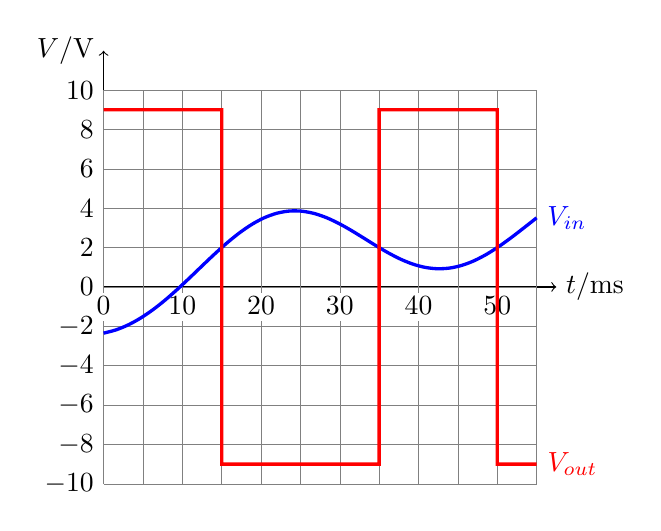
\begin{tikzpicture}
		\draw[->] (0,-2.5) -- (0,3) node[left]{$V$/V};
		\draw[->] (0,0) -- (5.75,0) node[right]{$t$/ms};
		\draw[step=0.5, gray, very thin] (0,-2.5) grid (5.5,2.5);
		\foreach \x in {0,10,...,50} {
			\draw[white,fill] (\x/10-0.2,-0.42) rectangle (\x/10+0.2,-0.08);
			\node[below] at (\x/10,0) {$\x$};
		}
		\foreach \y in {-10,-8,...,10} \node[left] at (0,\y/4) {$\y$};
		\draw [very thick,blue,domain=0:5.5,samples=36,smooth,variable=\x] plot (\x,{0.5+(\x-1.5)*(\x-3.5)*(\x-5)*exp(-0.15*(\x-3.5)*(\x-3))*0.2}) node[right]{$V_\text{in}$};
		\draw[very thick,red] (0,2.25) --++ (1.5,0) --++ (0,-4.5) --++ (2,0) --++ (0,4.5) -- (5,2.25) --++ (0,-4.5) -- (5.5,-2.25) node[right]{$V_\text{out}$};
		\end{tikzpicture}
	\end{minipage}
\end{figure}
	
\sol potential at non-inverting input: $V_+ = \frac{4.0}{4.0+6.0}\times(+5) = +2\text{ V}$

potential at inverting input is equal to input voltage: $V_-=V_\text{in}$

for $V_\text{in}$ greater than +2 V, $V_->V_+$, then $V_\text{out}=-9\text{ V}$

for $V_\text{in}$ less than +2 V, $V_-<V_+$, then $V_\text{out}=+9\text{ V}$

variation of $V_\text{out}$ can then be plotted, which shows the form of a square wave \eoe

\subsubsection{negative feedback}

in practical uses, we may desire $V_\text{out}$ to reflect small changes in $V_\text{in}$, instead of stuck at $\pm V_S$

there are a few problems with open-loop amplifiers that we need to deal with:

\begin{compactitem}
	\item[--] gain of amplifier is too high
	
	$V_\text{out}$ almost always saturates, so $V_\text{out}$ cannot change continuously with $V_\text{in}$
	
	\item[--] open-loop gain $G_0$ of practical op-amp is affected by temperature
	
	different $V_\text{out}$ for the same $V_\text{in}$ at different temperatures is not convenient
	
	\item[--] open-loop gain $G_0$ is a function of input frequency
	
	different input frequencies are not always amplified by same amount
	
	this would cause distortion of original signal, bandwidth would be limited
\end{compactitem}






one way to improve properties of amplifier circuits is to introduce negative feedback

feedback means sending a portion of output voltage back to the input terminals

a feedback network is also called a \emph{closed loop}

\begin{ilight}
	if a fraction of output $V_\text{out}$ is sent back to inverting input $V_-$ such that it opposes changes of input, this is called \keypoint{negative feedback}\index{negative feedback}\index{amplifier!negative feedback}
\end{ilight}

\begin{figure}[ht]
	\centering
	\begin{circuitikz}[european resistors]
		\draw[thick] (0,0) node[op amp] (opamp) {}
		(opamp.+) -- (-3.2,-0.5) node[left]{$V_+$}
		(opamp.-) -- (-2,0.5) -- (-2,2) -- (2,2) -- (2,0) (-2,0.5) -- (-3.2,0.5) node[left]{$V_-$}
		(opamp.out) -- (3,0) node[right]{$V_\text{out}$}
		(opamp.down) -- ++ (0,-.6) node[right] {$-V_S$}
		(opamp.up) -- ++ (0,.6) node[right] {$+V_S$};
		\draw[thick,blue,->] (1,2.4) [out=170,in=10] to (-1,2.4) ; 
		\node[blue,above] at (0,2.5) {$\beta V_\text{out}$};
	\end{circuitikz}

\caption*{negative feedback mechanism}
\end{figure}

let's look into the effect of introducing negative feedback into the amplifier circuit\footnote{Discussions in this section are not required by the syllabus. If you do not have the appetite, you may just skip to the conclusions.}

assume a fraction of output $\beta V_\text{out}$ ($0 < \beta \leq 1$) is fed back to inverting input of op-amp, then combined voltage to this terminal would be the sum of original $V_-$ and the feedback $\beta V_\text{out}$, the equation $V_\text{out} = G_0(V_+-V_-)$ for open-loop circuit shall be rewritten, hence we have



{
	
\centering
	
$V_\text{out} = G_0 \Big[( V_+ - (V_- + \beta V_\text{out})\Big]
\RA (1+G_0\beta)V_\text{out} = G_0(V_+ - V_-)
\RA V_\text{out} = \frac{G_0}{1+G_0\beta }(V_+ - V_-)$
	
}

overall gain of negative feedback amplifier is: $G=\frac{G_0}{1+ G_0\beta}$

this gain is less than open-loop gain $G_0$, so gain is reduced

further notice that $G_0\beta \gg 1$, we find $G \approx \frac{G_0}{\beta G_0} = \frac{1}{\beta}$

this shows for negative-feedback amplifier, as long as open-loop gain $G_0$ is sufficiently large, overall gain $G$ depends on $\beta$ only, i.e., only depends on how much output is sent back to $V_-$


$\beta$ can be controlled by a set of fixed resistors, which are not sensitive to change of frequency or temperature, so $G$ remains constant for a wider range of frequencies and temperatures




\newpage

we conclude that introducing negative feedback has the following benefits:

\begin{itemize}[leftmargin=\parindent]
	\item[$\circ$] reduced gain
	
	\item[$\circ$] more stable gain
	
	\item[$\circ$] increased bandwidth
	
	\item[$\circ$] less distortion
\end{itemize}


\subsubsection*{the golden rule}

with negative feedback, we expect that $V_\text{out}$ is able to change correspondingly with $V_\text{in}$

for any op-amp, $V_\text{out} = G_0(V_+-V_-)$, but op-amp has very large open-loop gain $G_0$

if $V_\text{out}$ does not saturate, one must have $V_+ - V_- \approx 0$

this can be summarised as the \emph{golden rule}: output of op-amp attempts to do whatever is necessary to make the difference between the two input voltages zero

note that op-amp can do this only if there is negative feedback

\subsubsection{inverting amplifier}

one type of widely-used amplifier circuit is called \keypoint{inverting amplifier}\index{amplifier!inverting amplifier}

\begin{figure}[htp]
\centering
\begin{circuitikz}[european resistors,scale=1.25]
	\draw[thick] (0,0) node[op amp] (opamp) {}
	(opamp.+) -- (-2,-0.4) -- (-2,-1.6) node[ground]{} 
	(opamp.-) -- (-2,0.4) to [R,l_=$R_\text{in}$] (-5,0.4) node[left]{$V_\text{in}$}
	(opamp.out) -- (3,0) node[right]{$V_\text{out}$}
	(opamp.down) -- ++ (0,-.6) node[right] {$-V_S$}
	(opamp.up) -- ++ (0,.6) node[right] {$+V_S$};
	\draw[thick] (2,0) -- (2,2) to[R,l_=$R_\text{f}$] (-2,2) -- (-2,0.4);
	\draw[-triangle 60] (-2.5,0.4) -- ++(.1,0) node[below]{$I_\text{in}$};
	\draw[-triangle 60] (-1.4,0.4) -- ++(.1,0) node[below]{$i$};
	\draw[-triangle 60] (-2,1.2) -- ++(0,.1) node[right]{$I_\text{f}$};
\end{circuitikz}
	
\caption*{inverting amplifier}
\end{figure}

$V_\text{out}$ is related to $V_\text{in}$ by $\boxed{V_\text{out} = \left(-\frac{R_\text{f}}{R_\text{in}}\right)V_\text{in} }$, where gain of the amplifier is $G=\frac{V_\text{out}}{V_\text{in}} = -\frac{R_\text{f}}{R_\text{in}}$
	
to show this relation, we need two approximations

\cmt virtual earth approximation: if $V_\text{out}$ does not saturate, must have $V_+ \approx V_-$, but $V_+$ is earthed, i.e., $V_+=0$, so $V_-\approx 0$, referred to as a \keypoint{virtual earth}

\cmt small current approximation: because of the very large input impedance of op-amp, current flowing into inverting input is negligible, i.e., $i\approx 0$

therefore currents through $R_\text{in}$ and $R_\text{f}$ are approximately the same: $I_\text{in} = I_\text{f}$

from this equation, we can relate $V_\text{out}$ to $V_\text{in}$:

{
	\centering
	
	$\frac{V_\text{in} - V_-}{R_\text{in}} = \frac{V_- - V_\text{out}}{R_\text{f}}
	\RA \frac{V_\text{in}-0}{R_\text{in}} = \frac{0-V_\text{out}}{R_\text{f}} 
	\RA V_\text{out} = \left(-\frac{R_\text{f}}{R_\text{in}}\right)V_\text{in}$
		
}

\subsubsection{non-inverting amplifier}

another type of common amplifier circuit is called \keypoint{non-inverting amplifier}\index{amplifier!non-inverting}

\begin{figure}[htp]
	\centering
	\begin{circuitikz}[european resistors,scale=1.25]
		\draw[thick] (0,0) node[op amp] (opamp) {}
		(opamp.+) -- (-1.9,-0.4) arc (0:180:0.1) -- (-3.6,-0.4) node[left]{$V_\text{in}$}
		(opamp.-) -- (-2,0.4) -- (-2,-1.6) to [R,l_=$R_\text{f}$] (2,-1.6) -- (2,0)
		(opamp.out) -- (3,0) node[right]{$V_\text{out}$}
		(opamp.down) -- ++ (0,-.6) node[right] {$-V_S$}
		(opamp.up) -- ++ (0,.6) node[right] {$+V_S$};
		\draw[thick] (-2,-1.6) -- (-2,-2.4) to[R,l_=$R_0$] (-2,-4) node[ground]{} ;
		\draw[-triangle 60] (-1.2,-1.6) -- ++(-.1,0) node[below]{$I_\text{f}$};
		\draw[-triangle 60] (-2,-2.2) -- ++(0,-.1) node[left]{$I_0$};
		\draw[-triangle 60] (-2,-1) -- ++(0,.1) node[left]{$i$};
	\end{circuitikz}
	
	\caption*{non-inverting amplifier}
\end{figure}

for this circuit, $V_\text{out}$ is given by: $\boxed{V_\text{out} = \left(1 + \frac{R_\text{f}}{R_0}\right)V_\text{in}}$, where overall gain $G=\frac{V_\text{out}}{V_\text{in}} = 1 + \frac{R_\text{f}}{R_0}$

to show this, recall current into input of op-amp $i\approx0$ due to its large input impedance, so

{

\centering
	
$I_\text{0} = I_\text{f} \RA \frac{V_- - 0}{R_0} = \frac{V_\text{out} - V_- -}{R_\text{f}}$

}


again, if $V_\text{out}$ is not saturated, $V_- \approx V_+ = V_\text{in}$, then we find


{
	
\centering

$\frac{V_\text{in}}{R_0} = \frac{V_\text{out} - V_\text{in}}{R_\text{f}} \RA  R_0 V_\text{out} - R_0 V_\text{in} = R_\text{f} V_\text{in}
\RA  V_\text{out} = \left(1 + \frac{R_\text{f}}{R_0}\right)V_\text{in}$
	
}

\subsubsection*{remarks on inverting \& non-inverting amplifiers}

inverting and non-inverting amplifiers are starting point for more complex circuits

before going through detailed examples, let's briefly comment on the results we have found
\begin{equation*}
	\text{for inverting amplifer: } G=\frac{-R_\text{f}}{R_\text{in}} \qquad \text{for non-inverting amplifer: } G=1+\frac{R_\text{f}}{R_0}
\end{equation*}

\cmt circuit's overall gain for both amplifiers only depend on choice of resistors

so gain can now be easily tuned, circuit design becomes more convenient

\cmt no parameter of op-amp shows up in final expressions for overall gain

gain is determined by feedback network, rather than by op-amp's characteristics
	
since value of resistors does not change significantly with temperature or frequency

this again means gain becomes now more stable with negative feedback
	
\cmt for inverting amplifiers, $G<0$, $V_\text{in}$ and $V_\text{out}$ always out of phase (opposite signs)
	
for non-inverting amplifiers, $G>0$, $V_\text{in}$ and $V_\text{out}$ always in phase (same sign)

\cmt the proportional relation between $V_\text{in}$ and $V_\text{out}$ only holds if op-amp is not saturated

if we find $V_\text{out}$ greater than supply voltage from a calculation, true $V_\text{out}$ equals $\pm V_S$



\example{In the inverting amplifier circuit below, $R_1=10$ k$\Omega$, $R_2=50$ k$\Omega$. (a) Find $V_\text{out}$ when $V_\text{in} = +1.0$ V. (b) Find $V_\text{out}$ when $V_\text{in} = -4.0$ V.}

\begin{figure}[ht]
	\centering
	\begin{circuitikz}[european resistors]
		\draw[thick] (0,0) node[op amp] (opamp) {}
		(opamp.+) -- (-2,-0.5) -- (-2,-1.5) node[ground]{} 
		(opamp.-) -- (-2,0.5) to [R,l_=$R_1$] (-5,0.5) node[left]{$V_\text{in}$}
		(opamp.out) -- (3,0) node[right]{$V_\text{out}$}
		(opamp.down) -- ++ (0,-.5) node[right] {$-10$V}
		(opamp.up) -- ++ (0,.5) node[right] {$+10$V};
		\draw[thick] (2,0) -- (2,2) to[R,l_=$R_2$] (-2,2) -- (-2,0.5);
	\end{circuitikz}
\end{figure}

\sol overall gain of the amplifier: $G=-\frac{R_2}{R_1} = -\frac{50\text{k}}{10\text{k}}=-5.0$

for $V_\text{in} = +1.0$ V: $V_\text{out}=(-5.0)\times(+1.0)=-5.0 \text{ V}$

for $V_\text{in} = -4.0$ V: $V_\text{out}=(-5.0)\times(-4.0)=+20 \text{ V}$, output becomes saturated, so $V_\text{out}=+10 \text{ V}$ \eoe


\newpage

\example{In the non-inverting amplifier circuit below, $R_1=48$ k$\Omega$, $R_2=6.0$ k$\Omega$. (a) Find $V_\text{out}$ when $V_\text{in} = +0.5$ V. (b) Find $V_\text{out}$ when $V_\text{in} = -3.0$ V.}

\begin{figure}[ht]
	\centering
	\begin{circuitikz}[european resistors,scale=1]
		\draw[thick] (0,0) node[op amp] (opamp) {}
		(opamp.+) -- (-1.9,-0.5) arc(0:180:0.1) -- (-3.6,-0.5) node[left]{$V_\text{in}$}
		(opamp.-) -- (-2,0.5) -- (-2,-1.6) to [R,l_=$R_1$] (2,-1.6) -- (2,0)
		(opamp.out) -- (3,0) node[right]{$V_\text{out}$}
		(opamp.down) -- ++ (0,-.5) node[right] {$-10$V}
		(opamp.up) -- ++ (0,.5) node[right] {$+10$V};
		\draw[thick] (-2,-1.6) -- (-2,-2.1) to[R,l_=$R_2$] (-2,-4) node[ground]{} ;
	\end{circuitikz}
\end{figure}

\sol overall gain of the amplifier: $G=1+\frac{R_1}{R_2} = 1+\frac{48\text{k}}{6.0\text{k}}=9.0$

for $V_\text{in} = +0.5$ V: $V_\text{out}=9.0\times(+0.5)=+4.5 \text{ V}$

for $V_\text{in} = -3.0$ V: $V_\text{out}=9.0\times(-3.0)=-27 \text{ V}$, output becomes saturated, so $V_\text{out}=-10 \text{ V}$ \eoe


\example{An amplifier circuit incorporating an ideal op-amp is shown.}

\begin{figure}[ht]
	\centering
	\begin{circuitikz}[european resistors,scale=1]
		\draw[thick] (0,0) node[op amp] (opamp) {}
		(opamp.+) -- (-2,-0.5) -- (-2,-2) node[ground]{} 
		(opamp.-) -- (-2,0.5) to [R,l_=$2.0\,k\Omega$] (-6,0.5) 
		(opamp.out) -- (3,0) node[right]{$V_\text{out}$}
		(opamp.down) -- ++ (0,-.6) node[right] {$-8\text{V}$}
		(opamp.up) -- ++ (0,.6) node[right] {$+8\text{V}$};
		\draw[thick] (2,0) -- (2,2) to[R,l_=$20\,k\Omega$] (-2,2) -- (-2,0.5);
		\draw[thick] (3,-2) -- (-6,-2) to [battery, l_=$1.0\text{V}$] (-6,0.5) ;
		\draw[->] (2.8, -2) --++(0,2);
		\draw[thick] (-2,2) -- (-2,3.6) to [thR,l=$R_T$] (2,3.6) -- (2,2);
	\end{circuitikz}
\end{figure}

Initially, the thermistor has a resistance of $20\,k\Omega$. (a) Find the gain of this circuit. (b) Find the output voltage. (c) State and explain how $V_\text{out}$ changes as temperature rises. (d) The thermistor is then removed, find the new output voltage.

\newpage

\solc \begin{compactitem}
	\item[(a)] this is an inverting amplifier (there is negative feedback loop and $V_\text{out}$ is fed into $V_-$)
	
	resistance of feedback loop: $R_\text{f} = \left(\frac{1}{20\text{k}} + \frac{1}{20\text{k}}\right)^{-1} = 10 \, \text{k}\Omega$
	
	\eqyskip gain of amplifer: $G= - \frac{R_\text{f}}{R_\text{in}} = -\frac{10\text{k}}{2.0\text{k}} \RA G=-5.0$
	
	\item[(b)] $V_\text{in}$ is at negative terminal of the battery, which is 1.0 V lower than the positive terminal
	
	but positive terminal is earthed, so $V_\text{in} = -1.0 \text{ V}$
	
	output voltage: $V_\text{out} = GV_\text{in} = (-5.0) \times (-1.0) \RA V_\text{out} = +5.0 \text{ V}$
	
	\item[(c)] as temperature increases, resistance of thermistor decreases
	
	total resistance of feedback loop becomes smaller
	
	gain of the circuit then becomes less negative, so $V_\text{out}$ will decrease
	
	\item[(d)] gain of amplifier after removal of thermistor: $G' = - \frac{R'_\text{f}}{R_\text{in}} = - \frac{20\text{k}}{2.0\text{k}} \RA G' = -10$
	
	new output voltage can be computed: $V'_\text{out} = G'V_\text{in} = (-10)\times(-1.0) = +10 \text{ V}$
	
	but voltage supply to op-amp is $\pm 8 \text{ V}$, op-amp saturates, so $V'_\text{out} = +8 \text{ V}$ \eoe
\end{compactitem}

\example{A circuit incorporating an ideal op-amp is shown below. The two fixed resistors have $R_1=36$ k$\Omega$ and $R_2=9.0$ k$\Omega$. Variation of $V_\text{in}$ from a voltage source is shown with the blue curve. On the same graph, plot how $V_\text{out}$ varies with time.}

\begin{figure}[ht]
	\begin{minipage}{0.52\textwidth}
		\centering
		\begin{circuitikz}[european resistors,scale=1]
			\draw[thick] (0,0) node[plain amp] (opamp) {}
			(opamp.-) -- (-2,0.5) -- (-3.5,0.5) to [sV] (-3.5,-4) -- (3,-4) 
			(opamp.+) -- (-2,-0.5) -- (-2,-1.8) to [R] (1.8,-1.8) -- (1.8,0)
			(opamp.out) -- (3,0)
			(opamp.down) -- ++ (0,-.6) node[right] {$-12$V}
			(opamp.up) -- ++ (0,.6) node[right] {$+12$V};
			\node at (-0.6,0.5) {$+$};
			\node at (-0.6,-0.5) {$-$};
			\draw[->] (2.7,-4) -- (2.7,0) node[midway, right]{$V_\text{out}$};
			\draw[thick] (-2,-1.6) -- (-2,-2.1) to[R,l^=$R_2$] (-2,-4) node[ground]{};
			\node at (0,-2.4) {$R_1$};
		\end{circuitikz}
	\end{minipage}\hfil
	\begin{minipage}{0.45\textwidth}
		\centering
		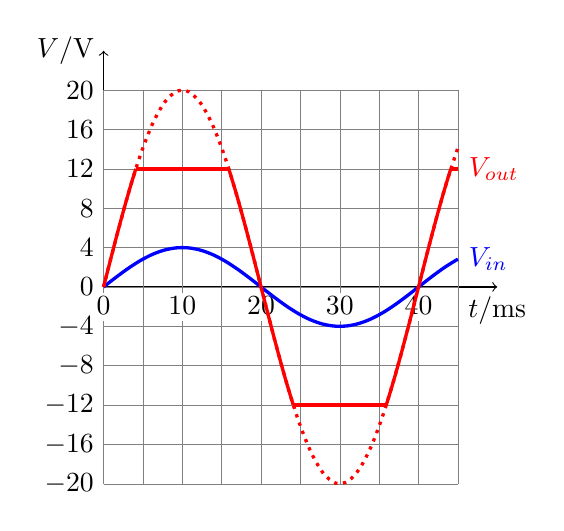
\begin{tikzpicture}
		\draw[->] (0,-2.5) -- (0,3) node[left]{$V$/V};
		\draw[->] (0,0) -- (5,0) node[below]{$t$/ms};
		\draw[step=0.5, gray, very thin] (0,-2.5) grid (4.5,2.5);
		\foreach \x in {0,10,...,40} {
			\draw[white,fill] (\x/10-0.2,-0.42) rectangle (\x/10+0.2,-0.08);
			\node[below] at (\x/10,0) {$\x$};
		}
		\foreach \y in {-20,-16,...,20} \node[left] at (0,\y/8) {$\y$};
		\draw [very thick,blue,domain=0:4.5,samples=30,smooth,variable=\x] plot (\x,{sin(\x*90)/2}) node[right]{$V_\text{in}$};
		\draw [very thick,red,dotted,domain=0:4.5,samples=30,smooth,variable=\x] plot (\x,{sin(\x*90)*2.5});
		\draw [very thick,red,domain=0:0.4097,samples=10,smooth,variable=\x] plot (\x,{sin(\x*90)*2.5});
		\draw [very thick,red,domain=1.5903:2.4097,samples=10,smooth,variable=\x] plot (\x,{sin(\x*90)*2.5});
		\draw [very thick,red,domain=3.5903:4.4097,samples=10,smooth,variable=\x] plot (\x,{sin(\x*90)*2.5});
		\draw[very thick,red] (0.4097,1.5) -- (1.5903,1.5) (2.4097,-1.5) -- (3.5903,-1.5) (4.4097,1.5) -- (4.5,1.5) node[right]{$V_\text{out}$};
		\end{tikzpicture}
	\end{minipage}
\end{figure}

\sol this is a non-inverting amplifier, whose voltage gain is: $G=1+\frac{R_1}{R_2} = 1+\frac{36\text{k}}{9.0\text{k}}=+5.0$

so $V_\text{out}=+5.0\times V_\text{in}$, with which we attempt to plot $V_\text{out}$ as the red dotted curve

but $V_\text{out}$ will saturate at voltage of power supply, which is $\pm 12$ V

taking this into account, we can plot the true $V_\text{out}$ as the red solid curve \eoe




\newpage

\question{An amplifier circuit is used to monitor light intensity. The magnitude of its gain is required to increase as light intensity	increases. Suggest how this can be done.}

\question{Show that the output voltage from an inverting amplifier is $V_\text{out} = \left( -\frac{R_\text{f}}{R_\text{in}}\right)V_\text{in} $.}

\question{Show that the output voltage from a non-inverting amplifier is $V_\text{out} = \left( 1+\frac{R_\text{f}}{R_0}\right) V_\text{in} $.}

\subsection{output devices}

\subsubsection{LED}

a \keypoint{diode}\index{diode} is a device that only allows current to flow in one direction

%am ideal diode has zero resistance when forward-biased, current easily flows through it
%\footnote{For practical diodes, when it is forward-biased, there exists a threshold voltage $V_0$ below which the diode does not conduct. For $V<V_0$, even the diode is connected in the correct direction, it stays off. But when $V>V_0$, resistance of diode drops to almost zero. There also exists a breaking voltage $V_\text{br}$. If p.d. across the diode is greater than $V_\text{br}$, the diode may break down.}
%
%when an ideal diode backward-biased, it has infinite resistance, no current can flow


\begin{wrapfigure}{R}{0.45\textwidth}
	\centering
	\vspace*{-8pt}
	\begin{circuitikz}[european resistors,scale=1]
		\draw[thick] (-1.5,0) to [leD-] (1.5,0);
	\end{circuitikz}
	
	\caption*{electric symbol for an LED}
	
	\vspace*{15pt}
	\begin{circuitikz}[european resistors,scale=0.9]
		\draw[thick] (2.5,0) to [leD-,l_=LED$_2$] (2.5,2) to [R,l_=$R$] (2.5,4.5);
		\draw[thick] (0,4.5) to [R,l_=$R$] (0,2) to [leD-,l_=LED$_1$] (0,0);
		\draw[thick] (-2.5,4.5) --++ (0.5,0) node[above, twoline]{$V_\text{out}$ from\\processor} -- (2.5,4.5);
		\draw[thick] (2.5,0) -- (-1,0) node[ground]{} -- (-2.5,0);
	\end{circuitikz}
	\vspace*{-15pt}
\end{wrapfigure}

\keypoint{LED}\index{LED}, or light-emitting diode, is able to give off light when current passes through it

LEDs are efficient light emitters and they come in many different colours

LEDs can therefore be used as indicators to show the \emph{polarity} of $V_\text{out}$ from processing units

a partial circuit incorporating two LEDs used as output devices is shown

when $V_\text{out}>0$, LED 1 emits light, LED 2 is off

when $V_\text{out}<0$, LED 2 emits light, LED 1 is off

protector resistors $R$ are included to ensure LED units not to be broken by large $V_\text{out}$



\subsubsection{relay}

\keypoint{relay}\index{relay} is an electromagnetic switch which enables the use of a current in one circuit (control circuit) to switch on another current in a second circuit (controlled circuit)

a relay consists of an electromagnet, a moveable arm and switch contacts

current flowing in the coils of the electromagnet induces a magnetic field to attract the moveable arm, which then connects the contacts and completes the second circuit

\cmt relay is used for many purposes, some of which are listed below

\begin{compactitem}
	\item[--] switching large voltage/current by means of a small voltage/current
	
	\item[--] high voltage isolation
	
	\item[--] remote switching
\end{compactitem}


\begin{figure}[ht]
	\centering
	\begin{circuitikz}[european resistors,scale=1.2]
		\draw[thick] (3,0) to [D-,l_=$D_1$] (3,-2) to [twoport] (3,-4)
		(1.5,-4) to [D-,l^=$D_2$] (1.5,-2) -- (3,-2);
		\draw[thick] (4,-4) -- (4,-3.2) -- (4.35,-2.5) (4,-2.4) -- (4,0);
		\draw[thick] (3,0) -- (0.6,0) node[above,twoline]{$V_\text{out}$ from\\control circuit} -- (0,0);
		\draw[thick] (4,0) -- (5.6,0) node[above,twoline]{controlled\\circuit} -- (6,0);
		\draw[thick] (0,-4) -- (5,-4) node[ground]{} -- (6,-4);
	\end{circuitikz}

	\caption*{output from processing units connected to a relay}	
\end{figure}

\cmt in practice, a relay is usually connected with two \emph{diodes} for the following reasons:

\begin{compactitem}
	\item[--] diode $D_1$ ensures relay is triggered only for positive $V_\text{out}$
	
	without $D_1$, relay would operate for currents flowing in either direction
	
	\item[--] diode $D_2$ protects sensitive processing units from large currents induced from relay coil
	
	when control circuit is turned off, large currents could be induced from relay coil
	
	this current might damage an op-amp or other sensitive components
	
	$D_2$ opens a path for induced current to flow (a short circuit across coil)
\end{compactitem}





\subsubsection{calibrated meters}

we can use sensing devices to monitor a specific physical quantity, say $x$

$x$ could be temperature, light level, sound intensity, etc.

change in $x$ would cause change in output voltage from the processing units

\begin{wrapfigure}{r}{0.45\textwidth}
	\centering
	\vspace*{-15pt}
	\begin{tikzpicture}
	\draw[<->] (0,4) node[left]{$V_\text{out}$} -- (0,0) -- (5,0) node[below]{$x$};
	\draw[thick, orange, domain=0.3:5,samples=36,smooth,variable=\x] plot (\x,{10/(\x+2)-0.8});
	\foreach \x in {0.6,1.4,1.9,2.6,3.7,4.3} \draw[thick] (\x-0.06,{10/(\x+2)-0.86}) --++ (0.12,0.12) ++ (0,-0.12) --++ (-0.12,0.12);
	\end{tikzpicture}
	\caption*{example of a calibration curve}
\end{wrapfigure}

for convenience, we would hope value of $x$ can be directly read off from a voltmeter, so we need associate a value of $V_\text{out}$ with a value for $x$

$V_\text{out}$ from processors is usually \emph{non-linear} in $x$, so one must \keypoint{calibrate} scale of meter in terms of $x$, 

calibration can be done according to a curve of measured data, called \emph{calibration curve}

scale will be non-uniform, but this is doable

\subsection{practical electronic circuits}

the many things we learned so far can be put together to build functional electronic circuits

in last part of this section, we will see a few examples of practical circuits


\subsubsection{automatic illumination system}

the circuit below enables automatic switching of lamp when it gets dark

\begin{figure}[ht]
	\centering
	\begin{circuitikz}[european resistors,scale=1.2]
		\draw[thick,->] (-3.05,-1.6) -- ++(-.3,-.3);
		\draw[thick,->] (-3.05,-1.4) -- ++(-.3,-.3);
		\draw[thick] (3,3)node[right] {$+V_S$} -- (-3.6,3)
		 (-3.6,.5) to [vR,l^=$R_\text{v}$] (-3.6,3)
		 (-3.6,.5) -- ++(0,-1) to [R,l_=LDR] ++(0,-2.5) -- ++ (7.1,0)node[ground]{} -- ++(3,0);
		\draw[thick] (-2,3) to [R,l_=$R_1$] (-2,.5) -- ++(0,-1) to [R,l_=$R_2$] ++(0,-2.5);
		\draw[thick] (0,0) node[op amp] (opamp) {}
		(opamp.+) -- (-1.9,-.417) arc(0:180:0.1) -- (-3.6,-.417) node[above right]{$A$}
		(opamp.-) -- (-2,.417) node[above right]{$B$}
		(opamp.out) -- (3,0) to[D-,l_=$D_1$] (3,-1.5) to [twoport] (3,-3)
		(1.5,-3) to [D-,l^=$D_2$] (1.5,-1.5) -- (3,-1.5)
		(opamp.down) -- ++ (0,-.6) node[right] {$-V_S$}
		(opamp.up) -- (0,3);
		\draw[thick] (4,-3) -- (4,-2.6) -- (4.35,-2) (4,-1.9) -- (4,0) to[lamp] ++(2.5,0) to[sV] ++(0,-3);
	\end{circuitikz}
\end{figure}

this circuit consists of a comparator, whose inputs are provided from two potential dividers

output from the comparator could trigger a relay that controls an illumination circuit

fixed resistors $R_1$ and $R_2$ provide a constant potential to $V_-$ for reference

magnitude of $V_+$ depends on the voltage share on LDR, which depends on light conditions

when in bright, LDR has low resistance, $V_+$ is low, so $V_+<V_-$, $V_\text{out}$ from op-amp is negative

current through relay is blocked by diode $D_1$, lamp circuit is off

as light level falls, resistance of LDR increases, $V_+$ then rises

at a certain light level, $V_+$ becomes greater than $V_-$, $V_\text{out}$ from op-amp becomes positive

current in relay triggers the switch to close, the lamp is switched on

variable resistor $R_\text{v}$ can be set to determine the critical light level of switch-over

\subsubsection{multi-range voltmeter}

the inverting amplifier can be adapted to make a multi-range voltmeter

positive connection of voltmeter is at $P$ so that positive reading is obtained for $+V_\text{in}$

\begin{figure}[htp]
	\centering
	\begin{circuitikz}[european resistors,scale=1]
		\draw[thick] (0,0) node[op amp] (opamp) {}
		(opamp.+) -- (-1.8,-0.5) -- (-1.8,-2.5) node[ground]{} 
		(opamp.-) -- (-3,0.5) (-3,1.8) -- (-3,-0.8)
		(opamp.out) -- (2.5,0) to[rmeter, t=V] (2.5,-2.5)
		(opamp.down) -- ++ (0,-.6) node[right] {$-V_S$}
		(opamp.up) -- ++ (0,.6) node[right] {$+V_S$};
		\foreach \y/\ytext in {1.8/500,0.5/5.0k,-0.8/50k}{
			\draw[thick] (-6,\y) to [R,l^={\ytext$\Omega$}] (-3,\y);
		}
		\foreach \y/\ytext in {1.8/A,0.5/B,-0.8/C}{
			\draw[fill=white] (-6,\y) circle (0.05) node[above] {$\ytext$};
		}
	
		\draw[thick] (1.5,0) -- (1.5,2.1) to[R,l_={50k$\Omega$}] (-2,2.1) -- (-2,0.5);
		\draw[thick] (-8.5,0.5) -- (-7,0.5) -- (-6,1.4);
		\draw[fill=white] (-7,0.5) circle(0.05);
		\draw[thick] (-8.5,-2.5) -- (2.5,-2.5);
		\draw[thick,->] (-8.1,-2.5) -- (-8.1,0.5) node[midway,right]{$V_\text{in}$};
		\node[right] at (2.5,-1.9) {P};
	\end{circuitikz}
\end{figure}

in this example, $V_\text{in}$ can be sent into the amplifier through three different channels

you can check that each channel has a different value of gain: $G_A = -100$, $G_B=-10$, $G_C=-1.0$

if the voltmeter connected to the output of op-amp has a range of $0\sim10$ V, then for $V_\text{in}$ less than $0.1$ V, or in the range $0.1\sim1.0$ V, or in the range $1.0\sim10$ V, they can be sent through channel $A$, $B$ or $C$ respectively to get a noticeable deflection on the voltmeter



\subsubsection{digital signal regenerator}\label{ch-regenerator}

the circuit given below can be used to regenerate a digital signal
\footnote{The use of digital signals in communication systems will be discussed in detail in \S\ref{digital-transmission}.}

suppose $D$ is a silicon diode which develops a p.d. drop of 0.7 V when it is forward biased 

\begin{figure}[ht]
	\centering
	\begin{circuitikz}[european resistors,scale=1]
		\draw[thick] (-6,-3) -- ++ (6,0)node[ground]{} -- (6,-3);
		\draw[thick] (-6,3) node[above]{+3.0V} -- (-2,3) to [R,l] (-2,.5) -- ++(0,-1) to [R] ++(0,-2.5);
		\draw[thick] (0,0) node[op amp] (opamp) {}
		(opamp.+) -- (-1.9,-.5) arc(0:180:0.1) -- (-5,-.5) node[above right]{$V_\text{in}$}
		(opamp.-) -- (-2,.5)
		(opamp.out)  to[D-,l^=$D$] (3.5,0) to [R,l_=$R_\text{L}$] (3.5,-3) (3.5,0) --++ (1.8,0)
		(opamp.down) -- ++ (0,-.8) node[right] {$-4.7$V}
		(opamp.up) --++ (0,0.8) node[right]{$+4.7$V};
		\node[left] at (-2.2,1.75) {$R_1=3.6$k$\Omega$};
		\node[left] at (-2.2,-1.75) {$R_2=1.8$k$\Omega$};
		\draw[thick,->] (5,-3) -- (5,0) node[midway, right]{$V_\text{out}$};
	\end{circuitikz}
\end{figure}

\begin{wrapfigure}{r}{0.5\textwidth}
	\centering
	\vspace*{-15pt}
	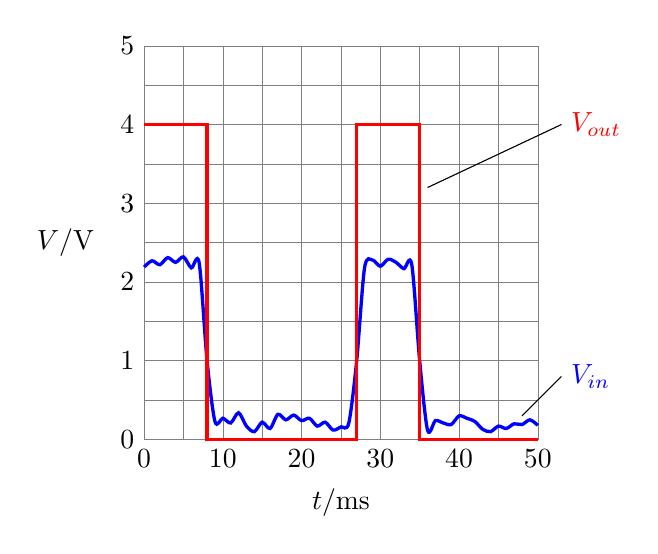
\begin{tikzpicture}
		\draw[step=0.5, gray, very thin] (0,0) grid (5,5);
		\foreach \x in {0,10,...,50} {
			\draw[white,fill] (\x/10-0.2,-0.42) rectangle (\x/10+0.2,-0.08);
			\node[below] at (\x/10,0) {$\x$};
		}
		\foreach \y in {0,1,...,5} \node[left] at (0,\y) {$\y$};
		\node at (2.5,-.8) {$t$/ms};
		\node at (-1,2.5) {$V$/V};
		\draw [blue, very thick] plot [smooth] coordinates {(0,2.19) (0.1,2.27) (0.2,2.22) (0.3,2.31) (0.4,2.25) (0.5,2.32) (0.6,2.18) (0.7,2.24) (0.8,1.0) (0.9,0.23) (1.0,0.27) (1.1,0.21) (1.2,0.34) (1.3,0.17) (1.4,0.10) (1.5,0.22) (1.6,0.14) (1.7,0.32) (1.8,0.25) (1.9,0.31) (2.0,0.24) (2.1,0.27) (2.2,0.17) (2.3,0.22) (2.4,0.12) (2.5,0.16) (2.6,0.21) (2.7,1.0) (2.8,2.18) (2.9,2.28) (3.0,2.20) (3.1,2.29) (3.2,2.25) (3.3,2.17) (3.4,2.22) (3.5,1.0) (3.6,0.12) (3.7,0.24) (3.8,0.21) (3.9,0.19) (4.0,0.30) (4.1,0.27) (4.2,0.23) (4.3,0.13) (4.4,0.10) (4.5,0.17) (4.6,0.14) (4.7,0.20) (4.8,0.19) (4.9,0.25) (5.0,0.18)} ;
		\draw (4.8,0.3) --++ (0.5,0.5) node[right] {\textcolor{blue}{$V_\text{in}$}};
		\draw[red,very thick] (0,4) -- (0.8,4) -- (0.8,0) -- (2.7,0) -- (2.7,4) -- (3.5,4) -- (3.5,0) -- (5,0);
		\draw (3.6,3.2) -- (5.3,4) node[right] {\textcolor{red}{$V_\text{out}$}};
	\end{tikzpicture}
	\vspace*{-25pt}
\end{wrapfigure}

$V_- = \frac{1.8}{1.8+3.6}\times(+3.0) = +1.0\text{ V}$ gives a constant potential to be compared with $V_+$

when $V_\text{in} > 1.0 \text{ V}$, i.e., $V_+>V_-$, output from op-amp is $ +4.7\text{ V}$, diode $D$ conducts and gets its voltage share of 0.7 V, the other 4.0 V is dropped across the load $R_\text{L}$, so $V_\text{out}=+4.0$ V

when $V_\text{in} < 1.0 \text{ V}$, i.e., $V_+<V_-$, output from op-amp is $ -4.7\text{ V}$, diode $D$ does not conduct, no current flows through $R_\text{L}$, then $V_\text{out}=0$

if a \emph{digital} signal is transmitted over a long distance, it may suffer from loss in power and noise, we would want to amplify the signal and remove the noise from it

this circuit can take in this signal and produce an output that removes the fluctuations due to noise and hence regenerates the original digital signal with only highs and lows

\subsubsection{summing amplifier}

circuits incorporating op-amp can carry out many mathematical operations

the circuit we are going to introduce here, called the \emph{summing amplifier}, is able to produce a voltage output as a \emph{weighted sum} of several input signals
\footnote{In a university-level electronic engineering course, you will see that op-amp can be used to build difference amplifiers, differentiator and integrator amplifiers (by including a capacitor), logarithmic amplifiers (by including a diode) and many other useful applications. Those who have interest in engineering science are encouraged to research on these topics.}

\begin{figure}[htp]
	\centering
	\begin{circuitikz}[european resistors,scale=1]
		\draw[thick] (0,0) node[op amp] (opamp) {}
		(opamp.+) -- (-1.8,-0.5) -- (-1.8,-2.5) node[ground]{} 
		(opamp.-) -- (-3,0.5) (-3,1.8) -- (-3,-0.8)
		(opamp.out) -- (2.5,0) to[rmeter, t=V] (2.5,-2.5)
		(opamp.down) -- ++ (0,-.6) node[right] {$-V_S$}
		(opamp.up) -- ++ (0,.6) node[right] {$+V_S$};
		\foreach \y/\ytext in {1.8/1,0.5/2,-0.8/3}{
			\draw[thick] (-7,\y) --++ (0.2,0) node[above]{$V_\ytext$} to [R,l^={$R_\ytext$}] (-3,\y); }
		\draw[thick] (-4,-2.5) -- (2.5,-2.5);
		\draw[thick] (1.5,0) -- (1.5,2.1) to[R,l_={$R_\text{f}$}] (-2,2.1) -- (-2,0.5);
		\node[right] at (2.5,-1.9) {P};
	\end{circuitikz}
\end{figure}

this is basically a variation of the inverting amplifier

it can be shown that the output voltage from op-amp is given by: $V_\text{out} = -R_\text{f}\left( \frac{V_1}{R_1} + \frac{V_2}{R_2} + \frac{V_3}{R_3} \right)$


positive connection of voltmeter is at $P$ so positive reading is obtained for $V_1, V_2, V_3>0$

so reading on voltmeter is: $V = R_\text{f}\left( \frac{V_1}{R_1} + \frac{V_2}{R_2} + \frac{V_3}{R_3} \right)$, a weighted sum of inputs $V_1$, $V_2$, and $V_3$

\cmt in the case where $R_1=R_2=R_3=R_\text{f}$, the reading simply becomes: $V=V_1+V_2+V_3$

this circuit produces the algebraic sum of the inputs, so it becomes a \emph{voltage adder}

\cmt in the case where $R_\text{f} = 4R_1 = 2R_2 = R_3$, the reading becomes: $V=4V_1 + 2V_2 + V_3$

if $V_1$, $V_2$, $V_3$ are only allowed to be 0 or 1, they can represent a three-bit binary number

this circuit can convert this binary number into its decimal value

so what we have here is a \emph{binary-to-decimal converter}

\newpage

\question{For the summing amplifier introduced, if $R_\text{f}=R_1=10$ k$\Omega$, $R_1=1.0$ k$\Omega$, and $R_3=100$ $\Omega$, find an expression for the voltage reading displayed on the voltmeter, and hence suggest the function of this circuit.}

\question{Design a non-inverting summing amplifier where the inputs are sent into the non-inverting input of the op-amp. ($\star$)}

\question{Design a circuit for a house such that a fire alarm can be automatically triggered when the temperature in the house becomes too high. ($\star$)}



